\documentclass[letterpaper,12pt]{article}
\usepackage{ifthen}
\usepackage{times}
\usepackage{amsmath}
\usepackage{amssymb}
\usepackage{helvet}
\usepackage{courier}
\usepackage{fancyheadings}
\usepackage{hyperref}
\usepackage{comment}
\pagestyle{fancy}
\usepackage{pmc}
\usepackage{graphicx}
\setlength\textwidth{6.5in}
\setlength\textheight{8.5in}

%%%%%%%%%%%%%%%%%%%%%%%%%%%%%%%%%%%%%%%%%%%%%%%%%%%%%%%%%%%%%%%%%%%%%%%%%%%%%%%%%%
% Special for e-unibus doc commands

\newcommand{\ForLater}{
\begin{center}
{\bf NOT FOR CURRENT VERSION}
\end{center}
}
\newcommand{\TBC}{\framebox{\textbf{TO BE COMPLETED}}}
\newcommand{\DISCUSS}{\Ovalbox {\bf \textcolor{red}{FOR DISCUSSION}}}
\newcommand{\Input}{\framebox{\textsf{in}}}
\newcommand{\Output}{\framebox{\textsf{out}}}
\newcommand{\debug}[1]{\textbf{debug start} #1 \textbf{debug finish}}
\newcommand{\inx}[1]{\emph{#1}}
\newtheorem{notation}{Notation}
\newtheorem{definition}{Definition}
\newtheorem{problem_statement}{Problem Statement}
\newtheorem{invariant}{Invariant}
\newtheorem{assumption}{Assumption}
\newtheorem{resource_string}{Resource String}
\newtheorem{testcase}{Test Case}
\newtheorem{note}{Note}
\newtheorem{specification}{Specification}
\newtheorem{caution}{Caution}
\newtheorem{prereq}{Pre-requisite}
\newtheorem{action}{Action}
\newtheorem{query}{Query}
\newcommand{\beq}{\begin{equation}} %% new, no conflict
\newcommand{\eeq}{\end{equation}} %% new, no conflict
\newcommand{\be}{\begin{enumerate}}
\newcommand{\ee}{\end{enumerate}}
\newcommand{\bi}{\begin{itemize}}
\newcommand{\ei}{\end{itemize}}
\newcommand{\bv}{\begin{verbatim}}
\newcommand{\ev}{\end{verbatim}}
\newcommand{\bd}{\begin{description}}
\newcommand{\ed}{\end{description}}
\newcommand{\bpre}{\begin{prereq}}
\newcommand{\epre}{\end{prereq}}
\newcommand{\bact}{\begin{action}}
\newcommand{\eact}{\end{action}}
\newcommand{\bs}{\begin{specification}}
\newcommand{\es}{\end{specification}}
\newcommand{\btc}{\begin{testcase}}
\newcommand{\etc}{\end{testcase}}
\newcommand{\bc}{\begin{caution}}
\newcommand{\ec}{\end{caution}}
\newcommand{\la}{\leftarrow}
\newcommand{\IpArgs}{\subsection{Input Arguments}}
\newcommand{\PreReqs}{\subsection{Pre-requisities}}
\newcommand{\Actions}{\subsection{Actions}}
\newcommand{\Coverage}{{\bf To test coverage.}}

%%%%%%%%%%%%%%%%%%%%%%%%%%%%%%%%%%%%%%%%%%%%%%%%%%%%%%%%%%%%%%%%%%%%%%%%%%%


\newtheorem{theorem}{Theorem}[section]
\newtheorem{lemma}[theorem]{Lemma}
\newtheorem{proposition}[theorem]{Proposition}
\newtheorem{corollary}[theorem]{Corollary}

\newenvironment{proof}[1][Proof]{\begin{trivlist}
\item[\hskip \labelsep {\bfseries #1}]}{\end{trivlist}}
\newenvironment{intuition}[1][Intuition]{\begin{trivlist}
\item[\hskip \labelsep {\bfseries #1}]}{\end{trivlist}}
%% \newenvironment{definition}[1][Definition]{\begin{trivlist}
%% \item[\hskip \labelsep {\bfseries #1}]}{\end{trivlist}}
\newenvironment{example}[1][Example]{\begin{trivlist}
\item[\hskip \labelsep {\bfseries #1}]}{\end{trivlist}}
\newenvironment{remark}[1][Remark]{\begin{trivlist}
\item[\hskip \labelsep {\bfseries #1}]}{\end{trivlist}}

\newcommand{\qed}{\nobreak \ifvmode \relax \else
      \ifdim\lastskip<1.5em \hskip-\lastskip
      \hskip1.5em plus0em minus0.5em \fi \nobreak
      \vrule height0.75em width0.5em depth0.25em\fi}

%%%%%%%%%%%%%%%%%%%%%%%%%%%%%%%%%%%%%%%%%%%%%%%%%%%%%%%%%%%%%%%%%
% \newcommand{\Alogon}{\mbox{\fontfamily{ptm}\selectfont {\large \selectfont A} \hspace{-1.2ex} {\large \selectfont L} \hspace{-2.3ex} \raisebox{0.45ex}{ {\footnotesize \selectfont O} } \hspace{-1.80ex} {\large \selectfont G} \hspace{-1.80ex} \raisebox{-0.33ex}{ {\large \selectfont O} } \hspace{-1.8ex} {\large \selectfont N}}}



\newcommand{\beq}{\begin{equation}} %% new, no conflict
\newcommand{\eeq}{\end{equation}} %% new, no conflict
\newcommand{\bdm}{\begin{displaymath}} %% new, no conflict
\newcommand{\edm}{\end{displaymath}} %% new, no conflict
% \newcommand{\reals}{{\rm I\! R}} %% new, no conflict
\newcommand{\reals}{\cal{R}} %% new, no conflict
\newcommand{\bb}[1]{\mathbf{#1}}
\newboolean{longform}
\setboolean{longform}{false}
\newboolean{blogpost}
\setboolean{blogpost}{true}
%% Another option is \usepackage{comment}
%% \includecomment(answer} or excludecomment{answer} % then
%% \begin{answer} ... \end{answer}


%% From https://math.berkeley.edu/~gbergman/misc/hacks/langl_rangl.html
\newcommand{\langl}{\begin{picture}(4.5,7)
\put(1.1,2.5){\rotatebox{60}{\line(1,0){5.5}}}
\put(1.1,2.5){\rotatebox{300}{\line(1,0){5.5}}}
\end{picture}}

\newcommand{\rangl}{\begin{picture}(4.5,7)
\put(.9,2.5){\rotatebox{120}{\line(1,0){5.5}}}
\put(.9,2.5){\rotatebox{240}{\line(1,0){5.5}}}
\end{picture}}

\newcommand{\mymean}[1]{\ensuremath{\langl{#1}\rangl}} %% new, no conflict

\begin{document}
\title{Duration of an AB test based on Power}
\author{Ramesh Subramonian, Ranjeet S. Tate, Michael Shire, Abhinav Singh}
\date{}
\maketitle
\thispagestyle{fancy}
\lhead{}
\chead{}
\rhead{}
\lfoot{}
% \cfoot{{\small NerdWallet Engineering }}
% \rfoot{{\small \thepage}}

\section{Introduction}
\label{sec:intro}
The fundamental question we want to answer here is: ``For how long should one run an AB test?''

There are two kinds of errors we want to reduce:
\be
\item False Positives or Type I errors (accepting something as good
  when it is actually bad). Let the probability of a False Positive
  (also known as the \(p\)-{\em value} be \(\alpha\). Typically
  \(\alpha\) is about \(0.05\).
\item False Negatives or Type II errors (rejecting something as bad
  when it is actually good). Let the probabiity of a False Negative be
  \(\beta\). This is related to the {\em power} as we discuss
  later. Typically \(\beta\) is about \(0.20\).
\ee

The power of a test is the proportion of errors which are False Negatives, since it is related to the discrimination with which you can detect small real effects. It is defined as
\bdm
    {\tt power} = \frac\beta{\alpha+\beta}
\edm
and so a typical value is \(80\%\).

For an A/B test, let \(X\) and \(Y\) be the values measured for each variant respectively. The variables are assumed (under the null hypothesis) to be independently distributed with the same mean and variance.
Let the comparison metric be
\(M(x,y)\) and let its mean
\beq
\mymean{M} = \mymean{M(x,y)}
\eeq
The two contrasting hypotheses are
\beq
\begin{split}
  H0&:\mymean{M} = 0\\
  H1&:\mymean{M} \ge \mu\\
\end{split}
\eeq

where \(\mu\) is the size of the effect we want to detect. For obvious reasons, its value is the same as the importance level we've used elsewhere.

If \(H1\) is true and we want the probability of Type I errors to be less than \(\alpha\) then the probability of Type II errors\footnote{Almost everything here is a slight generalization of the results in the Wikipedia article on ``Statistical Power'' \url{}.} is given by
\beq
B(\mu) \approx 1- \Phi(-z_\alpha -\frac{\mu}{\sigma_\mu})
\eeq
where \(\Phi()\) is the quantile function of the (normalized) normal distribution \(\Phi ={\tt norm.cdf(loc = 0, scale = 1)}\) so that
\beq
\begin{split}
  \Phi(-z_p) &=p\quad{\rm or}\\
  \Phi(z_p) &= 1-p
\end{split}
\eeq
and \(\sigma_\mu\) is the standard error in \(\mu\).

Inquiring minds want to know: {\em How much data do we need to keep the probability of Type II errors less than \(\beta\)?}

That is, we want
\beq\label{eq:bmu}
\begin{split}
 & B(\mu)<\beta \\
  \iff& 1-\beta < \Phi(-z_\alpha -\frac{\mu}{\sigma_\mu})\\
  \iff& -z_\alpha -\frac{\mu}{\sigma_\mu} < z_\beta\\
  \iff& \frac{\mu}{\sigma_\mu} > -z_\alpha -z_\beta
\end{split}
\eeq

\section{Example: Binary Valued Tests - Probability Difference}
Let \(p_A\) and \(p_B\) be the probabilities associated with a binary valued outcome, based on \(N_A\) and \(N_B\) trials respectively, and choose the probability difference as the comparison metric
\beq
M(p_A, p_B) = p_A-p_B >\mu
\eeq
Then,
\beq\label{eq:varmudiff}
\begin{split}
  var(\mu)&=\sigma^2_\mu = var(p_A) + var(p_B)\\
  &=\frac{p_A*(1-p_A)}{N_A} + \frac{p_B*(1-p_B)}{N_B}
  \end{split}
\eeq

Let \(p_A\approx p_B\approx p\) (the two probabilities are close and about equal to that of the Control group, which is the only probability we have some idea of ahead of time) and let \(N_A\approx N_B = \frac{N}{2}\), which is the optimum distribution for reducing the variance of the mean difference, as can be proven from the above Equation~\ref{eq:varmudiff}. Then
\beq
var(\mu) = 4*\frac{p*(1-p)}{N}
\eeq
Combining this with Equation~\ref{eq:bmu} we get
\beq
\frac{\mu\sqrt{N}}{2*\sqrt{p*(1-p)}} = -(z_\alpha+z_\beta)
  \eeq
  which in turn can be solved for the {\em total number of trials}
  \beq
  N> 4*(z_\alpha+z_\beta)^2*\frac{p*(1-p)}{\mu^2}
  \eeq

  \subsection{Numerical Example}
  Assume we've chosen close to typical values of \((\alpha,\beta) =(0.05, 0.10)\)
Using
\begin{table}
\centering
\begin{tabular}{|r|r|} \hline \hline
  {\bf -z} & {\bf 1-sided} \(\bb{p=1-\alpha}\) or \(\bb{1-\beta}\)\\
  \hline \hline
  1.3&0.10\\ \hline
  1.65&0.05\\ \hline
  2.35&0.01\\ 
  \hline\hline
\end{tabular}
\caption{\(z\) to \(p\)}
\label{table:ztop}
\end{table}
we have \(-(z_\alpha+z_\beta)\approx 3\), which yields
\beq
N>4*3^2*\frac{p*(1-p)}{\mu^2}
\eeq

If \(p=0.5\) and we have chosen a minimum important difference of \(0.10\), i.e. \(\mu = 0.10\), then \(N>900\).

If \(p\) is small, then we are looking for lift as a comparison metric. If we let \(\mu\) still be the difference in probabilities, then the lift is \(\frac{\mu}{p}\) and we can rewrite the above equation in terms of the number of conversions needed \(M\) as
\beq
M=p*N=\frac{36}{(\mu/p)^2}
\eeq
So if the conversion probability is small and we are lookig for a
moderate lift \(\frac{\mu}{p}=1\) then we need 36 conversions or
positives. If the effect we are looking for is small
\(\frac{\mu}{p}=0.1\), then we need \(3600\) conversions. So if a PM
wants to run a test ``just because'' or they are looking for a small
effect, they better justify the expense trying to get all the data.

\section{In parctise}
Any test has to be run for a week. If not, ask the PM to justify it on the grounds that day of week will {\em not} make a difference and why.

If the actual observed comparison metric turns out to be larger than \(\mu\), then you need {\em less data} to attain the same \((\alpha,\beta)\). This justifies building a {\em termination condition} into the AB server, to save on unneccesary testing costs.

\end{document}



\beq
\begin{split}
  <M> &\approx M(<x>,<y>)\\
  var(M) &\approx \left(\frac{\partial M}{\partial x}\right)^2\cdot var(x)
  + \left(\frac{\partial M}{\partial y}\right)^2\cdot var(y)
\end{split}
\eeq

\begin{figure}[ht!]
\centering
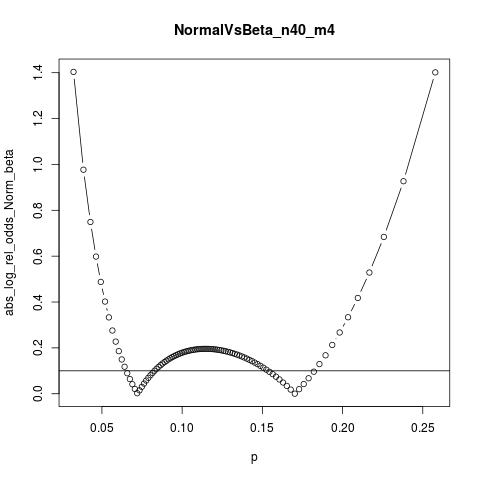
\includegraphics[width=90mm]{NormalVsBeta_n40_m4}
\caption{Comparing Cumulative Functions: Normal {\em not} a tolerable
approximation to \(\beta\) \label{fig:NormalVsBeta_40_4}}
\end{figure}
In Fig. \ref{fig:NormalVsBeta_40_4} we plot the absolute value of the log

\begin{table}
\centering
\begin{tabular}{|l|r|c|l|l|} \hline \hline
{\bf Metric} & {\bf Section} & {\bf Parameter} & \(\bb{M(x, y) > 0}\) & {\bf Boundary: }\(\bb{y = m(x)}\) \\ \hline \hline
Difference & \ref{sec:metric_diff} & \(\delta\) & \(x - y - \delta\)& \(y = x - \delta\) \\ \hline 
%
Lift & \ref{sec:metric_lift}& \(\lambda\) & \(x - y \cdot (1+\lambda)\) & \(y = \frac{x}{1+\lambda}\)\\ \hline 
%
Odds Factor & \ref{sec:metric_odds_factor} & \(\phi \)
& \(O(x)-\phi\cdot O(y)\)
  & \(y = O^{-1} \left( \frac{O(x)}{\phi}\right)\)\\ \hline
\hline
\end{tabular}
\caption{Summary of Metrics}
\label{table:metrics}
\end{table}
